In this chapter we are interested in the stationary 
Fokker-Planck equation
% \begin{equation}
% \begin{aligned}
\begin{align}
&\mathcal L p \stackrel{\rm def}{=}
  -\sum_{i=1}^d\frac{\partial(\mu_ip)}{\partial x_i} + \sum_{i=1}^d\sum_{j=1}^d\frac{\partial (D_{ij}p)}{\partial x_i\partial x_j}=0,\quad\mathbf x\in\mathbb R^d \label{eq:SFPE-0--steady-fp}\\
  &\int_{\mathbb R^d}p(\mathbf x)\,d\mathbf x = 1,\quad p(\mathbf x)\ge0\;\;\forall\;\mathbf x\in\mathbb R^d \nonumber
\end{align}
% \end{aligned}
% \end{equation}
Here $\mu\in C^1(\mathbb R^d; \mathbb R^d)$ is a non-solenoidal vector field, i.e., $\nabla\cdot\mu\not\equiv0$ in $\mathbb R^d$ and $\sigma\in C(\mathbb R^d; \mathbb R^{d\times d})$ is a matrix-valued function such that $D=\frac{1}{2}\sigma\sigma^\top$ is positive-definite.
The operator $\mathcal L$ is known as the \textit{Fokker-Planck operator} (FPO). The goal of this work is to devise an algorithm to find a non-trivial zero of  $\mathcal L$ in a mesh-free manner that works well in dimensions that are challenging for classical PDE-solvers. The motivations behind choosing to find a non-trivial zero of $\mathcal L$ rather than solving~\eqref{eq:SFPE-0--steady-fp}, as well as the motivation for restriction to non-solenoidal vector fields $\mu$, are as follows. 
\begin{itemize}
    \item Numerical integration suffers from the curse of dimensionality~\cite{hinrichs2014curse} and consequently the normalization constraint is extremely challenging to compute in high dimensions.
    \item One of the motivations is to devise an algorithm to solve time-dependent FPEs with unique solutions. We describe in a subsequent work~\cite{dynamicfp2024}, a method to find the normalized solution to the time-dependent FPE that uses a non-trivial zero of $\mathcal L$, even if is may be unnormalized.
    \item When $\mu$ is solenoidal, every constant function is a (unnormalized) zero of $\mathcal L$. In this case, we show in~\cite{dynamicfp2024} that if the corresponding time-dependent FPE has a unique solution, it may be obtained without using a non-trivial zero of $\mathcal L$ to calculate it. Hence we focus on non-solenoidal vector fields in this chapter.
    \item Lastly, rather than trying to force normalization during the computation of a non-trivial zero, it is much more economical to integrate the zero at the end to find the normalization constant at a one-time cost. Quasi Monte Carlo~\cite{leobacher2014introduction} or deep learning methods like i-flow~\cite{gao2020flow} can be used for this purpose. 
\end{itemize}
 

Although our method is valid for any matrix-valued $\sigma$ that gives rise to a positive definite $D$, in the demonstrations we use the form  $\sigma = a I_d$ where $a$ is a positive constant and $I_d$ is the $d\times d$ identity matrix. This allows us to abuse notation and use $\sigma$ and $D$ as scalar quantities. With this simplification our equation becomes, 
\begin{align}
    \mathcal L p= -\nabla\cdot(\mu p) + D\Delta p=0\label{eq:SFPE-1--steady-fp}
\end{align}
where $\Delta$ is the Laplacian operator. 

Since we approximate a solution to~\eqref{eq:SFPE-1--steady-fp} with a neural network, it is sensible to consider strong solutions. We therefore  restrict our search space of functions to $W^{1, 2}_{\rm loc}(\mathbb R^d)\cap C^2(\mathbb R^d)$. Since the superscripts for Sobolev spaces have been used interchangeably in literature, to avoid confusion we define $W^{1, 2}(\mathbb R^d)$ as
\begin{align}
    W^{1, 2}(\mathbb R^d) \stackrel{\rm def}{=} \{f\in L^2(\mathbb R^d):\|\nabla f\|_2\in L^2(\mathbb R^d)\}\label{eq:def-Sobolev--steady-fp}
\end{align} 
Sobolev spaces are frequently encountered while studying elliptic PDEs and therefore are very well-studied~\cite{brezis2011functional, kilpelainen1994weighted}.  This choice of function space enables us to prove uniqueness of solutions to the SFPEs that we will encounter in this chapter, as described in detail in appendix~\ref{ssec-unique--steady-fp}. Moreover, density of arbitrary-size neural networks in the space of continuous functions~\cite{pinkus1999approximation} and non-closedness of fixed-size neural networks in Sobolev spaces~\cite{mahan2021nonclosedness} are good justifications for our algorithm, as discussed in greater detail in section~\ref{ssec-infinite-to-finite--steady-fp}, making $W^{1, 2}_{\rm loc}(\mathbb R^d)\cap C^2(\mathbb R^d)$ an ideal function space to work with.

As mentioned earlier, one of the motivations for studying the SFPE is to device methods to find solutions of time-dependent FPE which occur quite often when studying time evolution of probability densities of random dynamical systems governed by stochastic differential equations of the form
\begin{align}
    x(t) = x(0) + \int_0^t \mu(x(s)) ds + \int_0^t \sigma(x(s)) dW(s) \,,
\label{eq-sde--steady-fp}\end{align} 
where $W(s)$ is a $d$-dimensional Brownian motion. We also refer to the related ODE system $\dot{x} = \mu(x)$ as the associated deterministic system and discuss the relation between the properties of this ODE, in particular, presence of a global attractor, and the solution of the SPFE.

\section{Examples}\label{sec-examples--steady-fp}
From an algorithmic perspective, it is important to have access to a class of equations on which our algorithm can be validated easily. Since classical methods do not work satisfactorily for our problem dimensions, the validating examples we use are those for which the analytical solutions are known. In addition to these examples, we also present results for which analytical solutions are not known. These example problems are described in this section.

\subsection{Gradient systems}
We first describe a very large class of systems for which analytical solutions can be written down, so that they can be used to validate the algorithms we propose. This class consists of equations where the drift $\mu$ can be written as the gradient of a potential function,
\begin{equation}
    \mu = -\nabla V \label{eq:mu-grad--steady-fp} \,.  
\end{equation}
To see why this structure of $\mu$ leads to analytical solutions of SFPEs, note that if $p=e^f$ is a solution to the SFPE then using~\eqref{eq:SFPE-1--steady-fp} \amit{we have $    \mathcal -\nabla\cdot(e^f\mu) + D\Delta e^f =0$, which gives
\begin{align}
    (\nabla + \nabla f)\cdot(\nabla (Df + V)) = 0 \,. \label{eq:log-factor-V--steady-fp}    
\end{align}
}
% %%%%%%
% [[[we have 
% \begin{align}
%     &\mathcal -\nabla\cdot(e^f\mu) + D\Delta e^f =0\\
%     \implies&  -\nabla\cdot \mu - \mu \cdot \nabla f + D\left(\|\nabla f\|_2^2 + \Delta f\right) =0 \label{eq:log-transform-0--steady-fp}\\
%     \implies&(\nabla + \nabla f)\cdot(D\nabla f -\mu) =0\label{eq:log-factor--steady-fp}\\
%     \implies&(\nabla + \nabla f)\cdot(\nabla (Df + V)) =0\label{eq:log-factor-V--steady-fp}    
% \end{align}]]]
% %%%%%%
Hence we can find one solution by simply setting the second term in the RHS of~\eqref{eq:log-factor-V--steady-fp} to be zero which gives us
\begin{align}
   p = c\exp\left(-\frac{V}{D}\right) \,,\label{eq:grad-sol--steady-fp}
\end{align}
% \begin{align}
%     &\nabla(Df + V) = \mathbf 0\\
%     \implies& f =\ln c-\frac{V}{D}\\
%     \implies& p= c\exp\left(-\frac{V}{D}\right)\label{eq:grad-sol--steady-fp}
% \end{align}
where $c$ is the normalizing constant. So a solution in this special case is already known up to the normalizing constant. We refer to a system satisfying~\eqref{eq:mu-grad--steady-fp} as a \textit{gradient system}.
In this chapter we use the following gradient systems to validate our algorithm in high dimensions. 

\subsubsection{2D ring system}
For $d=2$, $V=(x^2+y^2-1)^2$, and $\mu=-\nabla V$, we get the following SFPE,
\begin{align}
     4(x^2+y^2-1)\left(x\frac{\partial p}{\partial x}+y\frac{\partial p}{\partial y}\right) + 8(2x^2+2y^2-1)p + D\Delta p=0 \,. \label{eq:ring2D--steady-fp}
\end{align}
This system possesses a unique solution concentrated around the unit circle. The proof of uniqueness using the method of Lyapunov functions is given in the appendix~\ref{sssec-2D-unique--steady-fp}. The corresponding ODE system has the unit circle as a global attractor. This is a recurring theme in all of our example problems. Such systems with attractors are of great interest in the study of dynamical systems~\cite{ott1981strange} as well as filtering theory~\cite{kontorovich2009non}. We solve this system for $D=1$.

\subsubsection{2nD ring system} We can daisy-chain the previous system to build decoupled systems in higher dimensions. In this case the potential is given by
\begin{align}
    V(\mathbf x)=\sum_{i=0}^{\frac{d}{2}-1}(x_{2i}^2+x_{2i+1}^2-1)^2 \,,\qquad d=2n \,.
\end{align}
Since our algorithm does not differentiate between coupled and decoupled systems, this example serves as a great high-dimensional test case. In a subsequent work~\cite{dynamicfp2024}, we show how to solve the time-dependent FPEs with a method that is intimately related to the method presented in this chapter, and this system, being a decoupled high-dimensional system, presents a great way to verify the time-dependent algorithm. This is important since analytical solutions for time-dependent FPEs are not known in general even for gradient systems. Uniqueness of solution for the 2nD ring system directly follows from the uniqueness of solution for the 2D ring system, again thanks to its decoupled nature. In this chapter, we solve this system for $d = 4, 4, 6, 8, 10$ and with the choice of diffusion parameter $D=1$.

\subsection{Non-gradient Systems}
Not all the drifts $\mu$ can however be represented as the gradient of a potential. We call the systems belonging to this complementary class, \textit{non-gradient systems}. Analytic solutions for these systems are not known in general. Two examples of such systems that we use in this chapter are described below.

Since analytic solutions for non-gradient systems are not known, we restrict our attention to $d=3$ in this case. This is a dimension that can be reliably tackled with Monte Carlo simulations for comparison at a reasonable computational cost. See~\ref{ssec-MC-algo--steady-fp} for a description of the Monte Carlo algorithm that we use for such comparisons.

\subsubsection{Noisy Lorenz-63 system}
A famous example is the Lorenz-63 ODE system, first proposed by Edward Lorenz~\cite{lorenz1963deterministic} as an oversimplified model for atmospheric convection, with the drift $\mu$ given by
\begin{align}
    &\mu=[\alpha (y-x),\, x(\rho-z) - y,\, xy - \beta z]^\top \,, \label{eq:mu-L63--steady-fp}\\
    &\alpha = 10 \,, \, \beta = \frac{8}{3}\,, \, \rho=28 \,.
\end{align}
The well-known butterfly attractor associated with the corresponding ODE is shown in figure~\ref{fig:attractors--steady-fp}. 
\begin{figure}[t!]
    \centering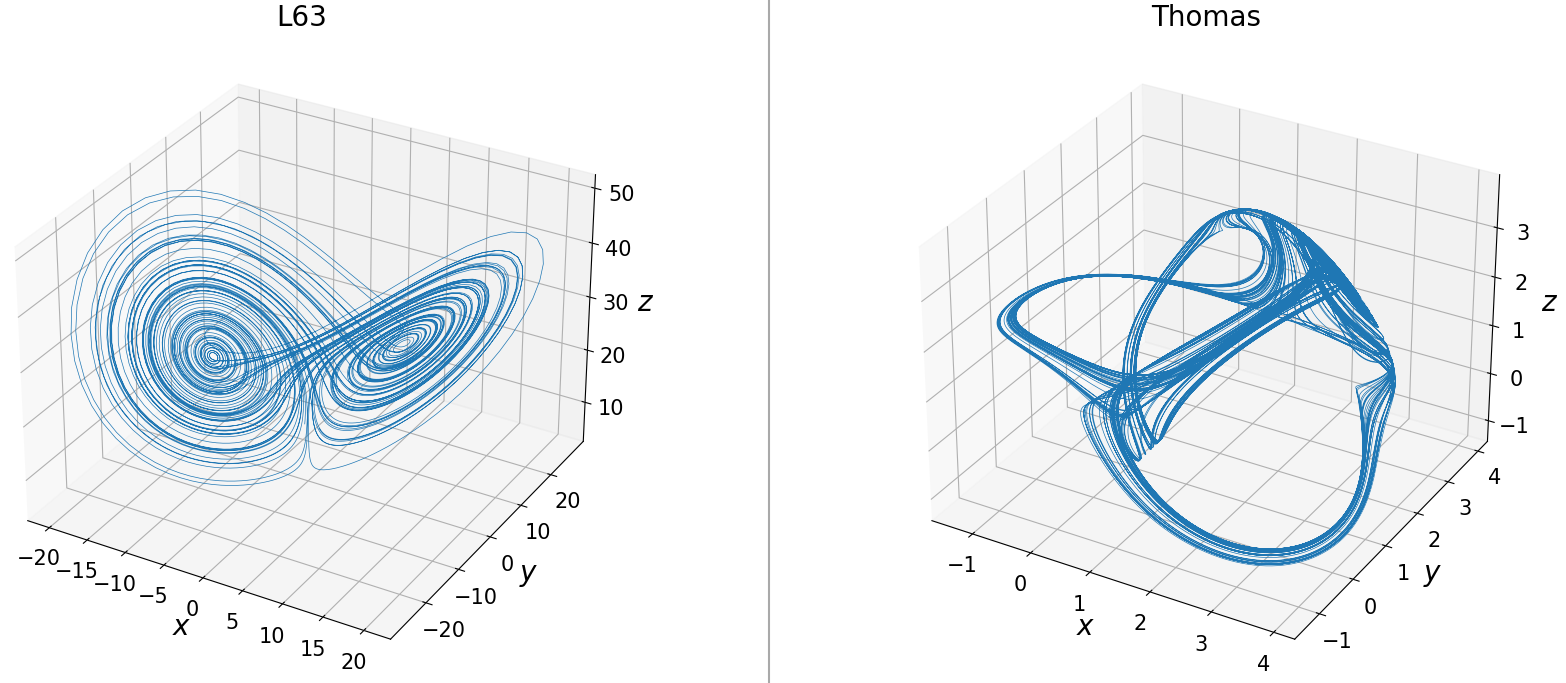
\includegraphics[scale=0.55]{steady-fp/plots/attractor.png}
   \caption{Attractors for non-gradient examples} \label{fig:attractors--steady-fp}
\end{figure}
This system and its variants like Lorenz-96 have become staple test problems in the field of data assimilation~\cite{carrassi2022data, yeong2020particle}. We use the standard parameters to define the drift and solve the system for $D=50$. This choice is motivated by the fact that this system already appears as a test case in~\cite{chen2018efficient}. With the choice of the drift $\mu(x)$ given above, the SFPE~\eqref{eq:SFPE-0--steady-fp} has a unique solution -- for a proof see appendix~\ref{sssec-L63-unique--steady-fp}.

\subsubsection{Noisy Thomas system}
Another example of a non-gradient system that we study is one for which the deterministic version was proposed by René Thomas~\cite{thomas1999deterministic}. It is a 3-dimensional system with cyclical symmetry in the three coordinates $x, y, z$ and the corresponding ODE system has a strange attractor which is depicted in figure~\ref{fig:attractors--steady-fp}.
We solve this system for $D=1$. The SFPE for this problem also has a unique solution -- for a proof see appendix~\ref{sssec-Thomas-unique--steady-fp}.
\begin{align}
    &\mu=[\sin y - bx,\, \sin z - by,\, \sin x - by ]^\top \,, \qquad b =  0.2 \,. \label{eq:mu-Thomas--steady-fp} 
\end{align}


